% !TeX program = tectonic
\documentclass[aspectratio=43]{beamer}
\usepackage[utf8]{inputenc}
\usepackage[T1]{fontenc}
\usepackage{lmodern}
\usepackage{amsmath, amssymb}
\usepackage{graphicx}
\usepackage{tikz}
\usetikzlibrary{arrows.meta,positioning,calc}
% Ensure figures auto-fit within slides by default
\setkeys{Gin}{width=\linewidth,height=0.62\textheight,keepaspectratio}
\usepackage{booktabs}
\usepackage{arydshln} % dashed lines in tables
\usepackage{array}    % advanced column types (m{...} for vertical centering)
\usepackage{hyperref}
\hypersetup{unicode=true}
% Sanitize PDF bookmarks: replace math/special macros with plain-text fallbacks
\pdfstringdefDisableCommands{%
  \def\textemdash{-}%
  \def\P{P}%
  \def\E{E}%
  \def\Var{Var}%
  \def\1{1}%
  \def\mathbb#1{#1}%
  \def\mathcal#1{#1}%
  \def\bm#1{#1}%
}
\usepackage{bm}
\usepackage{centernot} % for crossed implication symbols like \centernot\Rightarrow

% Notation and helpers
\newcommand{\R}{\mathbb{R}}
\renewcommand{\P}{\mathbb{P}}
\newcommand{\E}{\mathbb{E}}
\newcommand{\Var}{\operatorname{Var}}
\newcommand{\1}{\mathbf{1}}
\newcommand{\indep}{\perp\!\!\!\perp}
\newcommand{\toP}{\xrightarrow{\,\mathsf{P}\,}}
\newcommand{\toas}{\xrightarrow{\,\mathsf{a.s.}\,}}
\newcommand{\tod}{\xrightarrow{\,\mathcal{D}\,}}

% Helper for robust top-line commands (backup)
\newcommand{\robustcmd}[1]{\csname #1\endcsname}
% Provide a safe wrapper for text-formatting commands that may appear at line start
% Use \robustcmd{textbf}{...} where editors can strip a leading backslash accidentally.
\providecommand{\textbf}[1]{\robustcmd{textbf}{#1}}

\usetheme{Madrid}
\usecolortheme{default}
\setbeamertemplate{navigation symbols}{}

% Show a mini table of contents at the beginning of each section
\AtBeginSection[]{
  \begin{frame}{Outline}
  \robustcmd{tableofcontents}[currentsection,hideothersubsections]
  \end{frame}
}

\robustcmd{title}{Lesson 1 --- Statistical Modeling}
\robustcmd{subtitle}{Random Variables, Distributions, LLN, CLT}
\robustcmd{author}{Applied Statistics Course}
\robustcmd{date}{\today}

\begin{document}

\begin{frame}
  \robustcmd{titlepage}
\end{frame}

\section{Modeling Motivation}

% New: Modeling with Events \textemdash{} motivating examples
\begin{frame}{Why Probability? From Questions to Models}
  	\textbf{Natural language} \,\to\, \textbf{mathematical model} via events and random variables.
  \begin{itemize}
    \item Web A/B test: "Is variant B better than A?" $\Rightarrow$ Encode clicks as Bernoulli trials; compare $p_A$ vs $p_B$.
    \item Manufacturing: "Are defects random and rare?" $\Rightarrow$ Model counts with Poisson; check fit.
  \end{itemize}
  \medskip
  \begin{block}{Language of sets and probability}
    Events are sets (subsets of $\Omega$). Questions like "did a click occur?" or "defects $\le 3$" translate to $A\in\mathcal{F}$ and $\P(A)$.
  \end{block}
\end{frame}

\begin{frame}{From Natural Language to Events and RVs}{}
  {\small
  \centering
  % Increase row height for readability
  \renewcommand{\arraystretch}{1.30}%
  \setlength{\dashlinedash}{1pt}\setlength{\dashlinegap}{1.5pt}% dashed pattern
  \begin{tabular}{@{}m{0.32\textwidth} m{0.30\textwidth} m{0.32\textwidth}@{}}
    	\toprule
    	\textbf{Natural question} & \textbf{Event / RV} & \textbf{Typical model} \\
    \midrule
  "Roll of a fair die?" & \shortstack[l]{$X\in\{1,\dots,6\}$,\\ event $E=\{X\text{ even}\}$} & \shortstack[l]{$X$ uniform on $\{1,\dots,6\}$;\\ $\P(X=k)=1/6$} \\
    \addlinespace[3pt]
    \cdashline{1-3}
    \addlinespace[3pt]
  "User clicks?" & \shortstack[l]{$C=\{\text{click}\}$,\\ indicator $X=\1_C$} & \shortstack[l]{$X\sim\mathrm{Bernoulli}(p)$;\\ compare $p_A$ vs $p_B$} \\
    \addlinespace[3pt]
    \cdashline{1-3}
    \addlinespace[3pt]
  "Defects in a batch?" & Count $D\in\{0,1,2,\dots\}$ & \shortstack[l]{$D\sim\mathrm{Poisson}(\lambda)$\\ (rare, independent)} \\
    \addlinespace[3pt]
    \cdashline{1-3}
    \addlinespace[3pt]
  "Time until failure?" & Continuous $T\ge 0$ & \shortstack[l]{$T\sim\mathrm{Exponential}(\lambda)$\\ (memoryless)} \\
    \bottomrule
  \end{tabular}}
  \bigskip

  {
    \centering
    \small
    \begin{minipage}{0.9\linewidth}
      \centering
      	\textbf{Set operations encode logic:}\\ \alert{$A\cup B$} = "A or B",\enspace \alert{$A\cap B$} = "A and B"\\
      \alert{$A^c$} = "not A"
    \end{minipage}
  }
\end{frame}

\begin{frame}{Example: A/B Test as Bernoulli/Binomial}
  Each impression is a trial: click = 1, no click = 0. Variant-level CTR estimates $\hat p = \frac{\text{clicks}}{\text{impressions}}$.
  \begin{center}
    \includegraphics{figures/ab_test_ctr.png}
  \end{center}
  {\small Confidence intervals visualize uncertainty from finite samples.}
\end{frame}

\begin{frame}{Catchy: The Birthday Paradox}
  In a class of $n$ students, what's the chance at least two share a birthday? Surprisingly, at $n=23$ it's about 0.5.
  \begin{center}
    \includegraphics{figures/birthday_paradox.png}
  \end{center}
  {\small Shows how multiplicative complements and event counting yield unintuitive results.}
\end{frame}

\begin{frame}{Catchy: Monty Hall \textemdash{} Switch or Stay?}
  Game show setup: switching doors wins with probability $\approx 2/3$; simulation confirms the model.
  \begin{center}
    \includegraphics{figures/monty_hall.png}
  \end{center}
  {\small Encodes information and conditional probability; a great motivator for Bayes' rule.}
\end{frame}

\begin{frame}{Example: Defects as Poisson Counts}
  When events are rare and independent, counts in a fixed window often follow Poisson($\lambda$). Compare empirical distribution vs Poisson model.
  \begin{center}
  \includegraphics{figures/defects_poisson_by_batch.png}
  \end{center}
  {\small If the fit is reasonable, $\lambda$ summarizes the average defects per batch, guiding quality control.}
\end{frame}

\begin{frame}{Example: Time-to-Failure as Exponential}
  Waiting times between independent events are often modeled as Exponential($\lambda$). The survival is $S(t)=\P(T>t)=e^{-\lambda t}$.
  \begin{center}
    \includegraphics{figures/time_to_failure.png}
  \end{center}
  {\small Useful for reliability, queueing, and risk modeling.}
\end{frame}

\begin{frame}{Learning Objectives}
  \begin{itemize}
    \setlength{\itemsep}{0.45em}
    \item \textbf{Define random variables (RVs) and distributions}.\\[-0.25em]{\footnotesize Purpose: Map real-world uncertainty to mathematical objects and clarify what a distribution encodes.}
  \item \textbf{Use PMF/PDF/CDF to compute probabilities/quantiles}.\\[-0.25em]{\footnotesize Purpose: Turn event and threshold questions into computations to answer ``how likely?'' and ``what cutoff?''.}
    \item \textbf{Compute expectation, variance, and interpret moments}.\\[-0.25em]{\footnotesize Purpose: Summarize center and variability to compare models and quantify uncertainty/risk.}
    \item \textbf{Understand LLN and CLT (intuition + statements)}.\\[-0.25em]{\footnotesize Purpose: Explain why averages stabilize and when normal approximations apply, enabling CIs and tests.}
    \item \textbf{Connect descriptive statistics to probabilistic modeling}.\\[-0.25em]{\footnotesize Purpose: Bridge EDA to formal models so assumptions are explicit and limits understood.}
  \end{itemize}
\end{frame}

\section{Foundations and Random Variables}

% Main outline after first section has been declared (ensures items display)
% \begin{frame}{Outline}
%   \tableofcontents[hideallsubsections]
% \end{frame}

\begin{frame}{Probability Space}
  	\textbf{Definition.} A probability space is a triple $(\Omega,\,\mathcal{F},\,\P)$ where:
  \begin{itemize}
    \item $\Omega$ is the sample space; $\mathcal{F}\subseteq 2^{\Omega}$ is a $\sigma$-algebra;
    \item $\P:\mathcal{F}\to[0,1]$ is a probability measure, $\P(\Omega)=1$, and $\P$ is countably additive.
  \end{itemize}
  \medskip
  \begin{block}{Basic properties for events $A,B\in\mathcal{F}$}
    \begin{itemize}
      \setlength{\itemsep}{0.25em}
      \item Bounds: $0\le \P(A)\le 1$, with $\P(\varnothing)=0$ and $\P(\Omega)=1$.
      \item Complement: $\P(A^c)=1-\P(A)$.
      \item Monotonicity: $A\subseteq B\;\Rightarrow\; \P(A)\le \P(B)$.
      \item Union/intersection: $\P(A\cup B)=\P(A)+\P(B)-\P(A\cap B)$.
      \item Disjoint additivity: if $A\cap B=\varnothing$, then $\P(A\cup B)=\P(A)+\P(B)$; extends to countable disjoint unions.
    \end{itemize}
  \end{block}
  {\small Events are the measurable statements about outcomes: elements of $\mathcal{F}$.}
\end{frame}

\begin{frame}{Probability Space \textemdash{} Examples}
  \begin{exampleblock}{Examples}
    	\textbf{Fair coin (one toss):} $\Omega=\{H,T\}$, $\;\mathcal{F}=2^{\Omega}$, and $\;\P(\{H\})=\P(\{T\})=\tfrac12$. For $A=\{H\}$, $\P(A)=\tfrac12$, $\P(A^c)=\tfrac12$, $\P(A\cup A^c)=1$, $\P(A\cap A^c)=0$.
    \smallskip\newline
    	\textbf{Two fair tosses (illustrates independence):} $\Omega=\{HH,HT,TH,TT\}$ with $\P(\{\omega\})=\tfrac14$ for each outcome. Let $A$ be ``first toss is $H$'' $=\{HH,HT\}$ and $B$ be ``second toss is $H$'' $=\{HH,TH\}$. Then $\P(A)=\P(B)=\tfrac12$ and $\P(A\cap B)=\P(\{HH\})=\tfrac14=\P(A)\P(B)$, so $A$ and $B$ are independent.
  \end{exampleblock}
\end{frame}

\begin{frame}{Independence \textemdash{} a central notion}
  	\textbf{Events.} $A\indep B$ iff $\P(A\cap B)=\P(A)\,\P(B)$. More generally, a family $(A_i)$ is \emph{mutually independent} if $\P\!\big(\cap_{i\in I} A_i\big)=\prod_{i\in I}\P(A_i)$ for all finite $I$.
  \begin{itemize}
    \setlength{\itemsep}{0.35em}
    \item Stability: if $A\indep B$, then $A^c\indep B$, $A\indep B^c$, and $A^c\indep B^c$.
    \item Pairwise vs mutual: mutual independence $\Rightarrow$ pairwise independence, but pairwise independence $\centernot\Rightarrow$ mutual independence.
    \item Random variables: $X\indep Y$ iff $\P(X\in B,\,Y\in C)=\P(X\in B)\,\P(Y\in C)$ for all measurable sets $B,C$.
    \item Modeling: i.i.d. samples assume independence; Poisson processes and exponential waiting times hinge on independence assumptions; CLT and many estimators rely on it.
  \end{itemize}
  {\small Remember: independence encodes \emph{no information} between events/variables; it is a strong and testable assumption.}
\end{frame}

\begin{frame}{Probability Space \textemdash{} Visual}
  \centering
  % Venn-style diagram of events within a sample space rectangle
  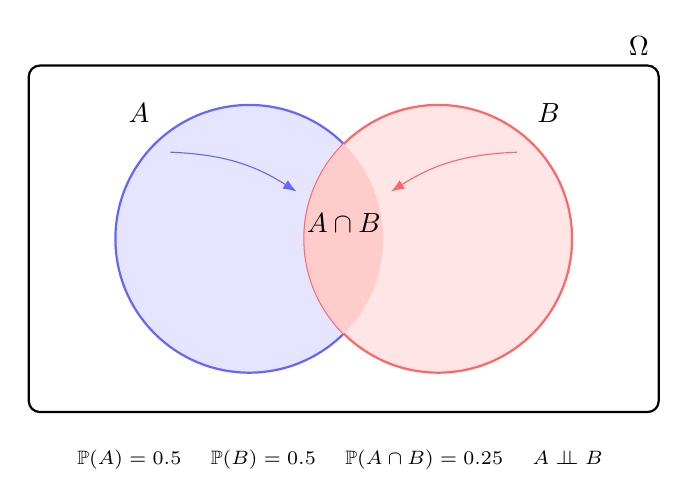
\begin{tikzpicture}[x=1cm,y=1cm]
    % Sample space rectangle
    \draw[rounded corners=4pt, thick] (-4,-2.2) rectangle (4,2.2);
    \node[anchor=south east] at (4,2.2) {$\Omega$};

  % Two events A and B (slightly smaller to create more whitespace)
  \def\eventrad{1.7}
  \filldraw[fill=blue!10, draw=blue!60, thick] (-1.2,0) circle (\eventrad);
  \filldraw[fill=red!10, draw=red!60, thick] (1.2,0) circle (\eventrad);

    % Intersection shading (A ∩ B)
    \begin{scope}
  \clip (-1.2,0) circle (\eventrad);
  \fill[red!20] (1.2,0) circle (\eventrad);
    \end{scope}

    % Labels
    \node at (-2.6,1.6) {$A$};
    \node at (2.6,1.6) {$B$};
    \node at (0,0.2) {$A\cap B$};

  % Example probabilities (illustrative) \textemdash{} lowered and smaller to avoid overlap
    \node[align=center, anchor=north, inner sep=2pt, fill=white, fill opacity=0.85, text opacity=1]
      at (0,-2.6) {\scriptsize
        $\P(A)=0.5\quad\ \P(B)=0.5\quad\ \P(A\cap B)=0.25\quad\ A\indep B$
      };

    % Decorative arrows to emphasize independence relation
    \draw[->, >=Latex, blue!60] (-2.2,1.1) to[bend left=15] (-0.6,0.6);
    \draw[->, >=Latex, red!60] (2.2,1.1) to[bend right=15] (0.6,0.6);
  \end{tikzpicture}

  \vspace{0.3em}
  {\small Visual intuition: events are subsets of $\Omega$; independence here matches $\P(A\cap B)=\P(A)\,\P(B)$.}
\end{frame}

\begin{frame}{Random Variables and Laws}{}
  {\small
  \begin{block}{Random variable}
    A real-valued random variable is a measurable map $X:(\Omega,\mathcal{F})\to(\R,\mathcal{B}(\R))$.
  \end{block}
  \vspace{-0.4em}
  \begin{block}{Law (distribution)}
    For $B\in\mathcal{B}(\R)$, the law of $X$ is the pushforward measure
    {\scriptsize\[
      \mu_X(B)=\P(X\in B)=\P\big(X^{-1}(B)\big).
    \]}
  \end{block}
  \vspace{-0.4em}
  \begin{block}{CDF (cumulative distribution function)}
    $F_X(x)=\P(X\le x)$. Properties: non-decreasing, right-continuous, $\lim_{x\to-\infty}F_X=0$, $\lim_{x\to\infty}F_X=1$.
  \end{block}
  \vspace{-0.4em}
  \begin{block}{Types of laws}
    Discrete (countable support; PMF $p_X$), absolutely continuous (PDF $f_X$; $F'_X=f_X$ a.e.), and mixed.
  \end{block}
  }
\end{frame}

\begin{frame}{Discrete random variables: PMF}{}
  {\small
  \begin{block}{What is a discrete RV?}
    $X$ takes values in a countable set $A=\{x_1,x_2,\dots\}$. Probability mass sits on points; probabilities \emph{add up} across values.
  \end{block}
  \vspace{-0.4em}
  \begin{block}{PMF (probability mass function)}
    The PMF $p_X(x)=\P(X=x)$ assigns a weight to each $x\in A$ with $p_X(x)\ge 0$ and $\sum_{x\in A} p_X(x)=1$. For any measurable $B$,
    {\scriptsize\[
      \P(X\in B)=\sum_{x\in A\cap B} p_X(x).
    \]}
    Interpretation: $p_X$ is a table (or bar chart) of \emph{weights} at allowed values.
  \end{block}
  % \vspace{-0.45em}
  % \begin{block}{Types of discrete variables}
  %   Nominal/categorical (unordered labels, e.g., color): PMF is appropriate; a CDF is not meaningful without an inherent order. Ordered/integer-valued (counts, ratings): both PMF and CDF apply because values are naturally ordered.
  % \end{block}
  % \vspace{-0.35em}
  {\scriptsize Examples: Bernoulli$(p)$: $p(1)=p$, $p(0)=1-p$.\quad Poisson$(\lambda)$: $p(k)=e^{-\lambda}\,\lambda^k/k!$, $k=0,1,2,\dots$.}
  }
\end{frame}

\begin{frame}{Discrete random variables: CDF}{}
  {\small
  \begin{block}{CDF (cumulative distribution function)}
    $F_X(x)=\P(X\le x)$ accumulates mass up to $x$. For discrete $X$, $F_X$ is a non-decreasing \emph{step} function; at each support point $x$ the jump size equals $p_X(x)$. Between support points $F_X$ is flat.
  \end{block}
  \vspace{-0.4em}
  \begin{block}{Using the CDF}
    For $a<b$,
    {\scriptsize\[
      \P(a< X\le b)=F_X(b)-F_X(a),\qquad \P(X=x)=F_X(x)-F_X(x^-)=p_X(x).
    \]}
    Properties: non-decreasing, right-continuous, $\lim_{x\to-\infty}F_X=0$, $\lim_{x\to\infty}F_X=1$.
  \end{block}
  \vspace{-0.45em}
  \begin{alertblock}{When is the CDF meaningful?}
    A CDF requires a meaningful order on the support. For nominal categories (unordered), prefer category probabilities (PMF); only define cumulative quantities once an inherent or agreed ordinal scale exists.
  \end{alertblock}
  }
\end{frame}

\begin{frame}{Continuous random variables: PDF}{}
  {\small
  \begin{block}{What is a continuous RV?}
    No atoms: $\P(X=a)=0$ for every $a\in\R$. Probabilities live on intervals/sets, not single points.
  \end{block}
  \vspace{-0.4em}
  \begin{block}{PDF (probability density function)}
    A nonnegative function $f_X$ with $\int_{\R} f_X(x)\,dx=1$ such that for any measurable $B$, $\P(X\in B)=\int_B f_X(x)\,dx$. For $a<b$,
    {\scriptsize\[
      \P(a< X\le b)=\int_a^b f_X(x)\,dx.
    \]}
  Intuition: $f_X$ is a \emph{height}; probability is \emph{area under the curve}. The PDF itself is not a probability.
  \end{block}
  \vspace{-0.35em}
  {\scriptsize Examples: Uniform$(a,b)$: $f=1/(b-a)$ on $[a,b]$; Exponential$(\lambda)$: $\lambda e^{-\lambda x}$ for $x\ge0$; Normal$(\mu,\sigma^2)$: bell-shaped.}
  }
\end{frame}

\begin{frame}{Continuous random variables: CDF}{}
  {\small
  \begin{block}{CDF (cumulative distribution function)}
    $F_X(x)=\P(X\le x)=\int_{-\infty}^{x} f_X(t)\,dt$. For $a<b$,
    {\scriptsize\[
      \P(a< X\le b)=F_X(b)-F_X(a)=\int_a^b f_X(x)\,dx.
    \]}
    Properties: non-decreasing, right-continuous, $\lim_{x\to-\infty}F_X=0$, $\lim_{x\to\infty}F_X=1$.
  \end{block}
  \vspace{-0.5em}
  \begin{alertblock}{Remember}
  The PDF is the \emph{derivative} of the CDF: $f_X(x)=F'_X(x)$ almost everywhere. The CDF is bounded in $[0,1]$; the PDF is a \emph{slope} and need not be $\le 1$ \textemdash{} probabilities come from \emph{areas} under $f_X$, not heights.
  \end{alertblock}
  \vspace{-0.5em}
  \begin{block}{Quantiles}
    For $q\in(0,1)$, a $q$-quantile is any $x$ with $F_X(x)\ge q$. If $F_X$ is strictly increasing, the $q$-quantile is $F_X^{-1}(q)$.
  \end{block}
  }
\end{frame}

\begin{frame}{Key Distributions (Discrete)}
  \begin{itemize}
    \item Bernoulli$(p)$: $\Pr(X=1)=p$, $\Pr(X=0)=1-p$, $\mathbb{E}[X]=p$, $\operatorname{Var}(X)=p(1-p)$
    \item Binomial$(n,p)$: sum of $n$ iid Bernoulli; $\mathbb{E}[X]=np$, $\operatorname{Var}(X)=np(1-p)$
    \item Poisson$(\lambda)$: $\Pr(X=k)=e^{-\lambda}\lambda^k/k!$, $\mathbb{E}[X]=\lambda$, $\operatorname{Var}(X)=\lambda$
  \end{itemize}
  \begin{center}
    \includegraphics[width=\linewidth,height=0.6\textheight,keepaspectratio]{figures/poisson_empirical_pmf.png}
  \end{center}
\end{frame}

\begin{frame}{Uniform (a, b)}{}
  {\footnotesize\begin{block}{Formulas}
    PDF: $f(x)=\begin{cases}\dfrac{1}{b-a}, & a\le x\le b,\\ 0, & \text{otherwise}\end{cases}$\quad
    CDF: $F(x)=\begin{cases}0, & x<a,\\ \dfrac{x-a}{b-a}, & a\le x\le b,\\ 1, & x>b\end{cases}$\\[0.4em]
    Mean: $\E[X]=\dfrac{a+b}{2}$\quad Variance: $\Var(X)=\dfrac{(b-a)^2}{12}$
  \end{block}}
  \begin{center}
    \includegraphics[width=\linewidth,height=0.45\textheight,keepaspectratio]{figures/uniform_density_cdf.png}
  \end{center}
\end{frame}

\begin{frame}{Exponential (\texorpdfstring{$\lambda$}{lambda})}{}
  {\footnotesize\begin{block}{Formulas}
    Support: $x\ge 0$\quad PDF: $f(x)=\lambda e^{-\lambda x}$\quad CDF: $F(x)=1-e^{-\lambda x}$\\[0.4em]
    Mean: $\E[X]=\dfrac{1}{\lambda}$\quad Variance: $\Var(X)=\dfrac{1}{\lambda^2}$\quad Memoryless: $\P(X>s+t\mid X>s)=e^{-\lambda t}$
  \end{block}}
  \begin{center}
    \includegraphics[width=\linewidth,height=0.45\textheight,keepaspectratio]{figures/exponential_density_cdf.png}
  \end{center}
\end{frame}

\begin{frame}{Normal (\texorpdfstring{$\mu,\sigma^2$}{mu, sigma^2})}{}
  {\footnotesize\begin{block}{Formulas}
    PDF: $f(x)=\dfrac{1}{\sigma\sqrt{2\pi}}\exp\!\Big(-\dfrac{(x-\mu)^2}{2\sigma^2}\Big)$\quad
    CDF: $F(x)=\Phi\!\Big(\dfrac{x-\mu}{\sigma}\Big)$ (no elementary closed form)\\[0.4em]
    Mean: $\E[X]=\mu$\quad Variance: $\Var(X)=\sigma^2$\quad Standardization: $\dfrac{X-\mu}{\sigma}\sim\mathcal{N}(0,1)$
  \end{block}}
  \begin{center}
    \includegraphics[width=\linewidth,height=0.45\textheight,keepaspectratio]{figures/normal_density_cdf.png}
  \end{center}
\end{frame}

\section{Moments and Convergence}

\begin{frame}{Expectation via measurable functions}{}
  {\small
  \begin{block}{Discrete case (PMF $p_X$)}
    For measurable $g$ with $\E[|g(X)|]<\infty$,
    \[ \E[g(X)] = \sum_{x\in\operatorname{supp}(X)} g(x)\,p_X(x) \quad \text{(absolute convergence).} \]
    In particular, take $g(x)=x$ to get $\E[X]=\sum_x x\,p_X(x)$.
  \end{block}
  \begin{block}{Continuous case (PDF $f_X$)}
    If $X$ admits a density $f_X$ w.r.t. Lebesgue measure and $\E[|g(X)|]<\infty$,
    \[ \E[g(X)] = \int_{\R} g(x)\, f_X(x)\, dx. \]
    In general, with law $\mu_X$, $\E[g(X)]=\int g\,d\mu_X$ (LOTUS). Setting $g(x)=x$ yields $\E[X]$.
  \end{block}
  }
  {\scriptsize Note: $\E[g(X)]$ is defined whenever $\int |g|\,d\mu_X<\infty$.}
\end{frame}

\begin{frame}{Expectation and variance: definitions and properties}
  \begin{block}{Definitions}
    For integrable $X$, the mean of the random variable is defined as
    \[ \E[X]=\int_\Omega X\,d\P=\int_{\R} x\,d\mu_X(x) \]
    If $\E[X^2]<\infty$, then the variance of the random variable is defined as
    \[ \Var(X)=\E\big[(X-\E[X])^2\big] = \E[X^2]-\E[X]^2. \]
  \end{block}
  \begin{alertblock}{Algebraic properties}
    \begin{itemize}
      \item Linearity: $\E[aX+b]=a\,\E[X]+b$ and $\E[X+Y]=\E[X]+\E[Y]$.
      \item Affine scaling: $\Var(aX+b)=a^2\Var(X)$; non-negativity: $\Var(X)\ge 0$ with equality iff $X$ is a.s. constant.
      \item Second-moment identity: $\Var(X)=\E[X^2]-\E[X]^2$ when $\E[X^2]<\infty$.
    \end{itemize}
  \end{alertblock}
\end{frame}

\begin{frame}{Higher-Order Moments: Skewness and Kurtosis}{}
  {\footnotesize
  \begin{block}{Definitions (when finite)}
    Let $\mu=\E[X]$, $\sigma^2=\Var(X)$, and central moments $\mu_k=\E\big[(X-\mu)^k\big]$. Skewness $\gamma_1:=\mu_3/\sigma^3$; Kurtosis $\beta_2:=\mu_4/\sigma^4$; Excess kurtosis $\gamma_2:=\beta_2-3$.
  \end{block}
  \vspace{-0.4em}
  \begin{block}{Relevance and interpretation}
    \begin{itemize}\setlength{\itemsep}{0.15em}
      \item Skewness ($\gamma_1$): \emph{asymmetry}. $\gamma_1>0$ right-skewed; $\gamma_1<0$ left-skewed; $\gamma_1=0$ for symmetric laws.
      \item Kurtosis ($\beta_2$) and excess ($\gamma_2$): tail weight/peakedness. Normal: $\beta_2=3$ hence $\gamma_2=0$.
      \item Practice: diagnose non-normality, tail risk, outlier propensity; both are outlier-sensitive (kurtosis especially).
      \item Sampling: for sample means, standardized skew decays $\propto n^{-1/2}$ and excess kurtosis $\propto n^{-1}$ (i.i.d., finite moments).
    \end{itemize}
  \end{block}
  }
\end{frame}

\begin{frame}{Example: Bernoulli (\texorpdfstring{$p$}{p})}
  \begin{block}{Random variable and summary}
    Let $X\sim\mathrm{Bernoulli}(p)$ with support $\{0,1\}$, $\P(X=1)=p$, $\P(X=0)=1-p$. Then $\E[X]=p$ and $\Var(X)=p(1-p)$.
  \end{block}
  \vspace{0.3em}
  	\textbf{Computation.}
  \begin{align*}
    \E[X] &= \sum_{x\in\{0,1\}} x\, p_X(x) = 0\cdot(1-p) + 1\cdot p = p. \\
    \E[X^2] &= \sum_{x\in\{0,1\}} x^2\, p_X(x) = 0^2\cdot(1-p) + 1^2\cdot p = p \quad (\text{since } X^2=X). \\
    \Var(X) &= \E[X^2] - (\E[X])^2 = p - p^2 = p(1-p).
  \end{align*}
\end{frame}

\begin{frame}{Example: Exponential (\texorpdfstring{$\lambda$}{lambda})}
  \begin{block}{Random variable and summary}
    Let $X\sim\mathrm{Exponential}(\lambda)$ with density $f_X(x)=\lambda e^{-\lambda x}\,\mathbf 1_{\{x\ge 0\}}$. Then $\E[X]=\dfrac{1}{\lambda}$ and $\Var(X)=\dfrac{1}{\lambda^2}$.
  \end{block}
  \vspace{0.3em}
  	\textbf{Computation.}
  \begin{align*}
    \E[X] &= \int_{0}^{\infty} x\, f_X(x)\, dx = \int_{0}^{\infty} x\, \lambda e^{-\lambda x}\, dx = \frac{1}{\lambda} \quad (\text{IBP or } \Gamma\text{ function}). \\
    \E[X^2] &= \int_{0}^{\infty} x^2\, f_X(x)\, dx = \int_{0}^{\infty} x^2\, \lambda e^{-\lambda x}\, dx = \frac{2}{\lambda^2}. \\
    \Var(X) &= \E[X^2] - (\E[X])^2 = \frac{2}{\lambda^2} - \frac{1}{\lambda^2} = \frac{1}{\lambda^2}.
  \end{align*}
\end{frame}

\begin{frame}{Example: Normal (\texorpdfstring{$\mu,\sigma^2$}{mu, sigma^2})}
  \begin{block}{Random variable and summary}
    Let $X\sim\mathcal N(\mu,\sigma^2)$ with density $f_X(x)=\dfrac{1}{\sigma\sqrt{2\pi}}\exp\!\Big(-\dfrac{(x-\mu)^2}{2\sigma^2}\Big)$. Then $\E[X]=\mu$ and $\Var(X)=\sigma^2$.
  \end{block}
  \vspace{0.3em}
  	\textbf{Computation.}
  Let $Z=\dfrac{X-\mu}{\sigma}\sim\mathcal N(0,1)$. Then
  \begin{align*}
    \E[X] &= \E[\mu + \sigma Z] = \mu + \sigma\, \E[Z] = \mu, \\
    \Var(X) &= \Var(\mu + \sigma Z) = \sigma^2\, \Var(Z) = \sigma^2 \quad (\Var(Z)=1).
  \end{align*}
\end{frame}

\begin{frame}{Moment Generating Function (MGF)}{}
  {\footnotesize
  \begin{block}{Definition}
    For a real-valued random variable $X$, the moment generating function (when finite) is
    \[
      M_X(t) = \E\big[e^{tX}\big], \qquad t\in D := \{t\in\R : \E[e^{tX}] < \infty\}.
    \]
  \end{block}
  \vspace{-0.35em}
  \begin{block}{Key properties and relevance}
    \begin{itemize}\setlength{\itemsep}{0.15em}
      \item Normalization: $M_X(0)=1$. If $M_X$ exists on a neighborhood of $0$, it uniquely determines the law of $X$.
      \item Moments: whenever $\E[|X|^k]<\infty$, $M_X^{(k)}(0)=\E[X^k]$.
      \item Affine and sums: $M_{aX+b}(t)=e^{bt}\,M_X(at)$; if $X\indep Y$, then $M_{X+Y}(t)=M_X(t)\,M_Y(t)$.
      \item Uses: identify distributions (e.g., Normal $M_X(t)=\exp(\mu t+\tfrac12\sigma^2 t^2)$), compute moments, and obtain distributions of sums of independent variables.
      \item Caveat: may fail to exist near $0$ for heavy-tailed laws (e.g., lognormal has $M_X(t)=\infty$ for $t>0$).
    \end{itemize}
  \end{block}
  }
\end{frame}

\begin{frame}{Characteristic Function}{}
  {\footnotesize
  \begin{block}{Definition}
    The characteristic function of $X$ is
    \[
      \varphi_X(t) = \E\big[e^{itX}\big], \qquad t\in\R.
    \]
  \end{block}
  \vspace{-0.35em}
  \begin{block}{Key properties and relevance}
    \begin{itemize}\setlength{\itemsep}{0.15em}
      \item Always exists; $\varphi_X(0)=1$, $|\varphi_X(t)|\le 1$; uniformly continuous and positive-definite.
      \item Uniqueness and inversion: $\varphi_X$ uniquely determines the law; inversion formulas recover the CDF/PDF under mild regularity.
      \item Moments: if $\E[|X|^k]<\infty$, then $\varphi_X^{(k)}(0)= i^k\,\E[X^k]$.
      \item Affine and sums: $\varphi_{aX+b}(t)= e^{ibt}\,\varphi_X(at)$; if $X\indep Y$, then $\varphi_{X+Y}(t)=\varphi_X(t)\,\varphi_Y(t)$.
      \item Limit theory: L\'evy continuity theorem links pointwise convergence of $\varphi_{X_n}$ to $X_n\tod X$; core tool for CLT and stable laws.
    \end{itemize}
  \end{block}
  }
\end{frame}

% --- New sequence: Modes of convergence (pedagogical) ---
\begin{frame}{Why Convergence Matters in Probability}
  \begin{itemize}
    \item Deterministic sequences: $a_n\to a$ means terms get arbitrarily close to a fixed limit.
    \item For random variables $(X_n)$, multiple notions of \emph{getting closer} exist.
    \item Hierarchy: \alert{a.s. $\Rightarrow$ in probability $\Rightarrow$ in distribution} (no converses in general).
  \end{itemize}
  \medskip
  {\centering
  % Visual placeholder: side-by-side deterministic vs random convergence
  \IfFileExists{figures/det_vs_random_convergence.png}{%
    \includegraphics{figures/det_vs_random_convergence.png}%
  }{%
    \fbox{\begin{minipage}{0.9\linewidth}\centering
      Placeholder: deterministic vs random convergence diagram (two panels)
    \end{minipage}}%
  }}
\end{frame}

\begin{frame}{Convergence Almost Surely}
  \begin{block}{Definition}
    \[ X_n \xrightarrow{\text{a.s.}} X \quad \iff \quad \mathbb{P}\big(\lim_{n\to\infty} X_n = X\big) = 1. \]
  \end{block}
  \begin{itemize}
    \item Intuition: \emph{pathwise} convergence for almost every outcome $\omega$.
    \item Strongest of the three: implies in probability (hence in distribution).
  \end{itemize}
  {\centering
  \IfFileExists{figures/as_convergence.png}{\includegraphics{figures/as_convergence.png}}{\fbox{\begin{minipage}{0.9\linewidth}\centering
    Placeholder: sample paths settling to a limit (a.s.)
  \end{minipage}}}}
  \medskip
  {\footnotesize Example: $X_n = X + Y\,\mathbf 1_{A}$ with $\P(A)=p$ small and fixed, and $Y\to 0$ deterministically. Then $X_n\toas X$ when the pathwise perturbations vanish almost surely.}
\end{frame}

\begin{frame}{Convergence in Probability}
  \begin{block}{Definition}
    \[ X_n \xrightarrow{\mathbb{P}} X \quad \iff \quad \forall \, \varepsilon > 0,\; \mathbb{P}(|X_n - X| > \varepsilon) \to 0. \]
  \end{block}
  \begin{itemize}
    \item Intuition: large deviations become rare; individual paths may still oscillate.
    \item Weaker than a.s.; stronger than in distribution (in general settings).
  \end{itemize}
  {\centering
  \IfFileExists{figures/in_prob_convergence.png}{\includegraphics{figures/in_prob_convergence.png}}{\fbox{\begin{minipage}{0.9\linewidth}\centering
    Placeholder: histograms narrowing around the target value
  \end{minipage}}}}
  \medskip
  {\footnotesize Example: $X_n=\mathbf 1_{\{U\le 1/n\}}$ with $U\sim\mathrm{Uniform}(0,1)$. Then $X_n\toP 0$ but $X_n\not\toas 0$.}
\end{frame}

\begin{frame}{Convergence in Distribution}
  \begin{block}{CDF-based definition}
    \[ X_n \xrightarrow{d} X \quad \iff \quad F_{X_n}(t) \to F_X(t) \; \text{ at all continuity points of } F_X. \]
  \end{block}
  \begin{block}{Portmanteau (equivalent)}
    \[ X_n \xrightarrow{d} X \quad \iff \quad \E[f(X_n)] \to \E[f(X)] \quad \text{for all bounded, \emph{continuous} } f. \]
  \end{block}
  \begin{itemize}
    \item Converging \emph{shape} of the distribution; samples need not get close pointwise.
    \item Do not replace ``continuous'' by ``measurable''; that would demand a stronger mode.
  \end{itemize}
  {\centering
  \IfFileExists{figures/in_dist_convergence.png}{\includegraphics{figures/in_dist_convergence.png}}{\fbox{\begin{minipage}{0.9\linewidth}\centering
    Placeholder: CDFs aligning across $n$
  \end{minipage}}}}
  \medskip
  {\footnotesize Example: Central Limit Theorem: $\sqrt{n}(\bar X_n-\mu)\tod \mathcal N(0,\sigma^2)$.}
\end{frame}

\begin{frame}{Comparing the Modes}
  \begin{itemize}
    \item Hierarchy: \alert{$X_n\toas X \Rightarrow X_n\toP X \Rightarrow X_n\tod X$}.
    \item Converses fail in general; classic counterexamples below.
  \end{itemize}
  {\small
  \renewcommand{\arraystretch}{1.25}
  \begin{tabular}{@{}lccc@{}}
    	\toprule
    Sequence $X_n$ (limit $X$) & a.s. & in $\mathsf P$ & in $\mathcal D$ \\
    \midrule
    $\mathbf 1_{\{U\le 1/n\}} \to 0$ & $\centernot\checkmark$ & $\checkmark$ & $\checkmark$ \\
    $X_n\equiv X$ and $Y=1-X$ & \textemdash & $\centernot\checkmark$ & $X_n\tod X$ and $X_n\tod Y$ \\
    Typewriter sequence $\to 0$ & $\centernot\checkmark$ & $\checkmark$ & $\checkmark$ \\
    \bottomrule
  \end{tabular}}
  \medskip
  {\centering
  \IfFileExists{figures/convergence_table.png}{\includegraphics{figures/convergence_table.png}}{\fbox{\begin{minipage}{0.9\linewidth}\centering
    Placeholder: table/chart summarizing which convergences hold
  \end{minipage}}}}
\end{frame}

\begin{frame}{Summary \& Intuition Map}
  {\small
  \renewcommand{\arraystretch}{1.25}
  \setlength{\dashlinedash}{1pt}\setlength{\dashlinegap}{1.5pt}
  \begin{tabular}{@{}m{0.16\linewidth} m{0.34\linewidth} m{0.24\linewidth} m{0.12\linewidth} m{0.10\linewidth}@{}}
    	\toprule
    	\textbf{Mode} & \textbf{Definition} & \textbf{Meaning} & \textbf{Visual} & \textbf{Implies} \\
    \midrule
    a.s. & $\P(\lim X_n=X)=1$ & Pathwise for a.e. outcome & sample paths settle & in $\mathsf P$ \\
    \cdashline{1-5}
    in $\mathsf P$ & $\P(|X_n-X|>\varepsilon)\to 0$ & Large deviations vanish & histograms narrow & in $\mathcal D$ \\
    \cdashline{1-5}
    in $\mathcal D$ & $F_{X_n}\to F_X$ (cont. pts) & Laws converge & CDFs align & \textemdash \\
    \bottomrule
  \end{tabular}}
  \medskip
  {\centering
  \IfFileExists{figures/summary_table.png}{\includegraphics{figures/summary_table.png}}{\fbox{\begin{minipage}{0.9\linewidth}\centering
    Placeholder: compact summary table/diagram
  \end{minipage}}}}
  \medskip
  \begin{block}{Takeaway}
    Stronger $\Rightarrow$ more pathwise closeness; weaker $\Rightarrow$ distribution-level agreement only.
  \end{block}
\end{frame}

\begin{frame}{Descriptive Statistics (Samples)}
  \begin{itemize}
    \item Sample mean $\bar x$, sample variance $s^2$, quantiles (median, IQR)
    \item Robustness: median (robust) vs mean (sensitive to outliers)
  \end{itemize}
  \begin{center}
    \includegraphics{figures/descriptive_stats.png}
  \end{center}
\end{frame}

\section{Limit Theorems}

\begin{frame}{Law of Large Numbers (LLN)}
  \textbf{Weak LLN.} If $X_1,X_2,\ldots$ are i.i.d. with $\E[X_i]=\mu$, then $\bar X_n=\tfrac{1}{n}\sum_{i=1}^n X_i \toP \mu$.
  \medskip
  \textbf{Strong LLN.} If $X_i$ are i.i.d. with $\E[|X_i|]<\infty$, then $\bar X_n \toas \mu$.
  \medskip
  \textbf{Sketch.} If $\Var(X_i)=\sigma^2<\infty$, then $\Var(\bar X_n)=\sigma^2/n$ and Chebyshev yields WLLN. Strong LLN follows under integrability via Kolmogorov.
  \begin{block}{Implication}
    Consistency of the sample mean; frequency interpretations; Monte Carlo convergence.
  \end{block}
\end{frame}

\begin{frame}{Central Limit Theorem (CLT)}
  \textbf{Lindeberg--L\'evy CLT.} If $X_1,\ldots,X_n$ are i.i.d. with $\E[X_i]=\mu$ and $\Var(X_i)=\sigma^2\in(0,\infty)$, then
  \[
    \sqrt{n}\,(\bar X_n-\mu) \tod \mathcal{N}(0,\sigma^2),\quad\text{equivalently}\quad \frac{\bar X_n-\mu}{\sigma/\sqrt{n}}\tod \mathcal{N}(0,1).
  \]
  \textbf{Generalizations.} Lyapunov and Lindeberg--Feller conditions allow independent, non-identically distributed sequences.
  \begin{block}{Implications}
    Large-sample normal approximations for estimators; construction of confidence intervals and tests.
  \end{block}
  \begin{exampleblock}{Bernoulli example}
    If $X_i\sim\mathrm{Bernoulli}(p)$, then $\hat p=\bar X_n$ satisfies $\sqrt{n}(\hat p-p)\tod \mathcal{N}(0, p(1-p))$.
  \end{exampleblock}
\end{frame}

\begin{frame}{Convergence: Examples to Contrast Modes}{}
  {\footnotesize
  \begin{itemize}
    \item $\toP$ but not $\toas$: independent $X_n\in\{0,1\}$ with $\P(X_n=1)=1/n$, limit $X\equiv 0$. Then $X_n\toP 0$ but $\P(X_n\to 0)=0$ (infinitely many ones a.s.).
    \item $\tod$ but not $\toP$: let $X\sim \mathrm{Bernoulli}(1/2)$ and $Y=1-X$. Then $X_n\equiv X$ tends to both $X$ and $Y$ in distribution, but $X_n\not\toP Y$.
    \item Typewriter sequence: $X_n(\omega)=\1_{[k2^{-m},(k+1)2^{-m}]}(\omega)$ for $n=2^m+k$; then $X_n\to 0$ in probability and in $L^p$ ($p<\infty$), but not a.s.
  \end{itemize}}
\end{frame}

\section{Worked Examples}

\begin{frame}{Examples}
  \begin{itemize}
    \item PMF vs empirical frequencies (Poisson counts)
    \item PDFs and shapes (Uniform/Exponential/Normal)
    \item QQ plots for normality (heights)
  \end{itemize}
  \begin{center}
    \includegraphics[width=\linewidth,height=0.65\textheight,keepaspectratio]{figures/heights_qq.png}
  \end{center}
\end{frame}

\section{Exercises}

\begin{frame}{Exercises (Theory)}
  \begin{enumerate}
    \item If $X\sim \mathrm{Uniform}(0,1)$, compute $\E[X]$, $\Var(X)$, median, and $q_{0.9}$.
    \item If $X\sim \mathrm{Poisson}(3)$, compute $\P(X\le 1)$ and $\E[X(X-1)]$.
    \item Show that for $X\sim \mathrm{Bernoulli}(p)$, skewness $\gamma_1 = \dfrac{1-2p}{\sqrt{p(1-p)}}$.
    \item Prove WLLN using Chebyshev for i.i.d. with finite variance.
  \end{enumerate}
\end{frame}

\begin{frame}{Practical Preview}
  \begin{itemize}
    \item EDA on heights dataset
    \item CLT simulation; Poisson fit to defects
  \end{itemize}
  \begin{block}{Reference}
    See practical tasks in the lesson materials and starter code in the repository.
  \end{block}
\end{frame}

\section{Summary and References}

\begin{frame}{Summary}
  \begin{itemize}
    \item Bridge descriptive to probabilistic modeling
  \end{itemize}
\end{frame}

\begin{frame}{References}
  \begin{itemize}
    \item Casella and Berger, Statistical Inference
    \item Wasserman, All of Statistics
    \item Grimmett and Stirzaker, Probability and Random Processes
  \end{itemize}
\end{frame}

\end{document}
